%% Plato FSM Translation Tech Memo
%% Design flow

\section {Design Flow \label{sec:design-flow}} 

\begin{figure}[H]
	\begin{centering}
		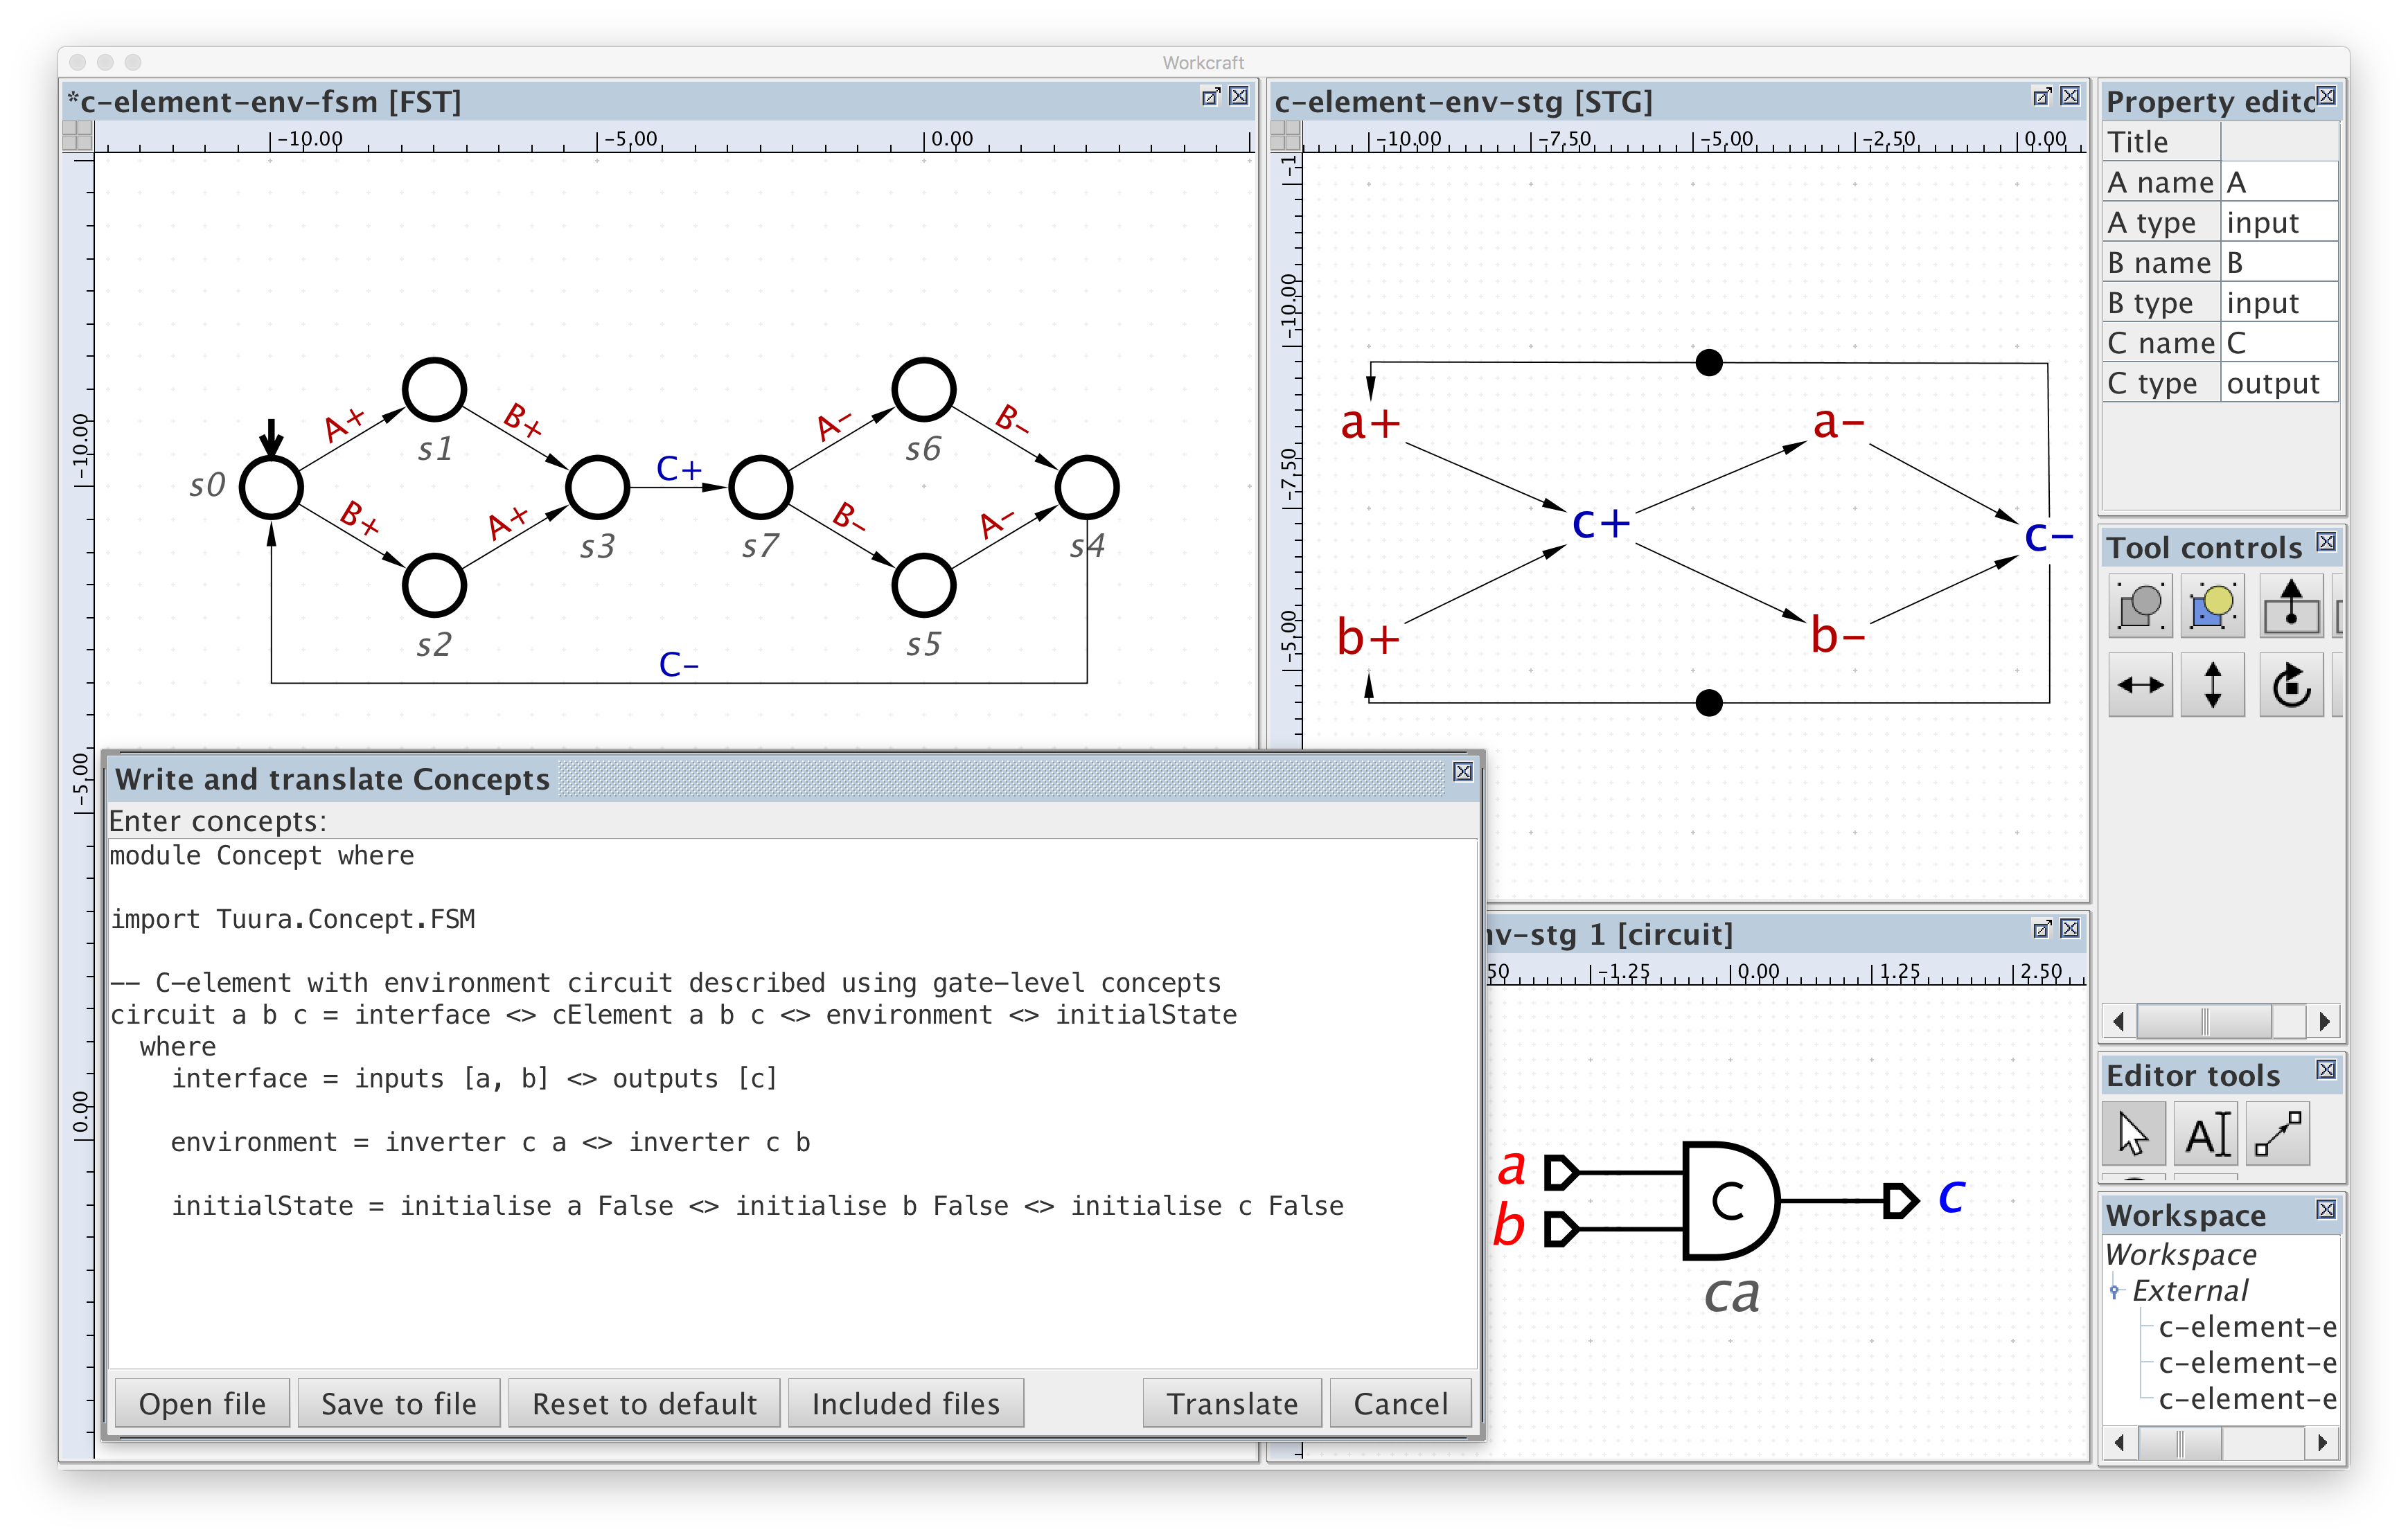
\includegraphics[scale=0.25]{images/workcraft-screenshot}
		\par\end{centering}
	\protect\caption{\label{fig:workcraft-screenshot} Example design flow in Workcraft}
\end{figure}

\noun{Plato} can be used as a command line tool, where a user can translate a concept specification, 
referencing the filepath, and importing other concept files which contain concepts used by the file to be 
translated. This will provide a user with an FSM or STG in a file format, .sg or .g respectively. These file 
formats can be used my many other tools to perform further operations on the translated models. 
 
It is also integrated into \noun{Workcraft}, an open-source tool-suite which also contains
several other back-end tools. This provides a GUI for visualising multiple modelling formalisms,
and for verification and synthesis of these models, and a visualisation of asynchronous circuits. For 
\noun{Plato} specifically, it provides the ability to directly import concept specifications as STGs, to 
write and save concept specifications, as well as open and edit existing concept files, and a window to 
select which files should be included in the translation process, in the event that the current 
specification uses concepts defined in other concept files. 

Figure~\ref{fig:workcraft-screenshot} contains an example of the design flow using \noun{Plato} from 
within \noun{Workcraft}. The bottom left contains the concepts authoring window. 
Above this is the FSM translated from 
the written concept specification, the same as seen in Figure~\ref{fig:c-element-env-fsm}. The top right 
contains the STG translated from the exact same concept specification, which is also the same as seen 
in Figure~\ref{fig:c-element-env-stg}. This STG can then be verified and synthesized using the back-end 
tools of \noun{Workcraft}, and synthesis will produce the actual gate of the C-element, as shown in the 
bottom-right of the image. 
